%%%%%%%%%%%%%%%%%%%%%%%%%%%%%%%%%%%%%%%%%
% Beamer Presentation
% LaTeX Template
% Version 1.0 (10/11/12)
%
% This template has been downloaded from:
% http://www.LaTeXTemplates.com
%
% License:
% CC BY-NC-SA 3.0 (http://creativecommons.org/licenses/by-nc-sa/3.0/)
%
%%%%%%%%%%%%%%%%%%%%%%%%%%%%%%%%%%%%%%%%%

%----------------------------------------------------------------------------------------
%	PACKAGES AND THEMES
%----------------------------------------------------------------------------------------

\documentclass{beamer}

\mode<presentation> {

% The Beamer class comes with a number of default slide themes
% which change the colors and layouts of slides. Below this is a list
% of all the themes, uncomment each in turn to see what they look like.

%\usetheme{default}
%\usetheme{AnnArbor}
%\usetheme{Antibes}
%\usetheme{Bergen}
%\usetheme{Berkeley}
%\usetheme{Berlin}
%\usetheme{Boadilla}
%\usetheme{CambridgeUS}
%\usetheme{Copenhagen}
%\usetheme{Darmstadt}
%\usetheme{Dresden}
%\usetheme{Frankfurt}
%\usetheme{Goettingen}
%\usetheme{Hannover}
%\usetheme{Ilmenau}
%\usetheme{JuanLesPins}
%\usetheme{Luebeck}
\usetheme{Madrid}
%\usetheme{Malmoe}
%\usetheme{Marburg}
%\usetheme{Montpellier}
%\usetheme{PaloAlto}
%\usetheme{Pittsburgh}
%\usetheme{Rochester}
%\usetheme{Singapore}
%\usetheme{Szeged}
%\usetheme{Warsaw}

% As well as themes, the Beamer class has a number of color themes
% for any slide theme. Uncomment each of these in turn to see how it
% changes the colors of your current slide theme.

%\usecolortheme{albatross}
%\usecolortheme{beaver}
%\usecolortheme{beetle}
%\usecolortheme{crane}
%\usecolortheme{dolphin}
%\usecolortheme{dove}
%\usecolortheme{fly}
%\usecolortheme{lily}
%\usecolortheme{orchid}
%\usecolortheme{rose}
%\usecolortheme{seagull}
%\usecolortheme{seahorse}
%\usecolortheme{whale}
%\usecolortheme{wolverine}

%\setbeamertemplate{footline} % To remove the footer line in all slides uncomment this line
%\setbeamertemplate{footline}[page number] % To replace the footer line in all slides with a simple slide count uncomment this line

%\setbeamertemplate{navigation symbols}{} % To remove the navigation symbols from the bottom of all slides uncomment this line
}

\usepackage{graphicx} % Allows including images
\usepackage{booktabs} % Allows the use of \toprule, \midrule and \bottomrule in tables
\usepackage{wrapfig}

%----------------------------------------------------------------------------------------
%	TITLE PAGE
%----------------------------------------------------------------------------------------

\title[Femtocell Simulations]{MATLAB Based Femtocell Network Simulation} % The short title appears at the bottom of every slide, the full title is only on the title page

\author{Travis Collins} % Your name
\institute[WPI] % Your institution as it will appear on the bottom of every slide, may be shorthand to save space
{
Worcester Polyntechnic Institute \\ % Your institution for the title page
\medskip
\textit{traviscollins@wpi.edu} % Your email address
}
%\date{\today} % Date, can be changed to a custom date
\date{January 23, 2015}

\begin{document}

\begin{frame}
\titlepage % Print the title page as the first slide
\end{frame}

\begin{frame}
\frametitle{Overview} % Table of contents slide, comment this block out to remove it
\tableofcontents % Throughout your presentation, if you choose to use \section{} and \subsection{} commands, these will automatically be printed on this slide as an overview of your presentation
\end{frame}

%----------------------------------------------------------------------------------------
%	PRESENTATION SLIDES
%----------------------------------------------------------------------------------------

%------------------------------------------------
\section{LTE Basics} % Sections can be created in order to organize your presentation into discrete blocks, all sections and subsections are automatically printed in the table of contents as an overview of the talk
%------------------------------------------------

%\subsection{} % A subsection can be created just before a set of slides with a common theme to further break down your presentation into chunks

%------------------------------------------------

\begin{frame}
  \frametitle{LTE Attributes/Features}
  \begin{itemize}
    \item LTE uses a fully scheduled MAC Layer (except for RACH)
    \item LTE comes in flavors of both TDD and FDD (FDD will be focused on since it can be simplier to evaluate and explain)
    \item Bandwidths from 1.4MHz to 20MHz
    \item Resource Blocks can be QPSK, 16QAM, 64QAM
    \item Turbocoding rates from 1/2 to 948/1024 (Puncturing when necessary)
  \end{itemize}
\end{frame}

%------------------------------------------------

\begin{frame}
\frametitle{Basic LTE Resource Allocation}
\begin{center}
  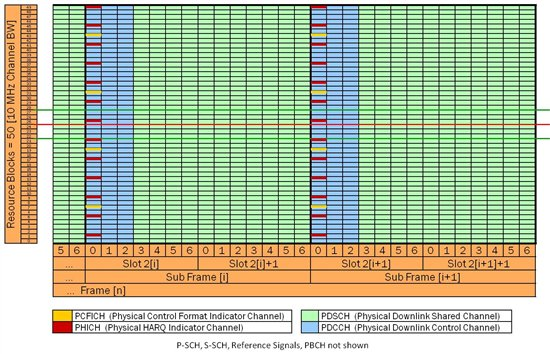
\includegraphics[width= 0.8\linewidth]{images/lte_frame.jpg}
\end{center}
\end{frame}

%------------------------------------------------

\begin{frame}
  \frametitle{Cell Topologies}
  \begin{center}
  \begin{figure}
    \centering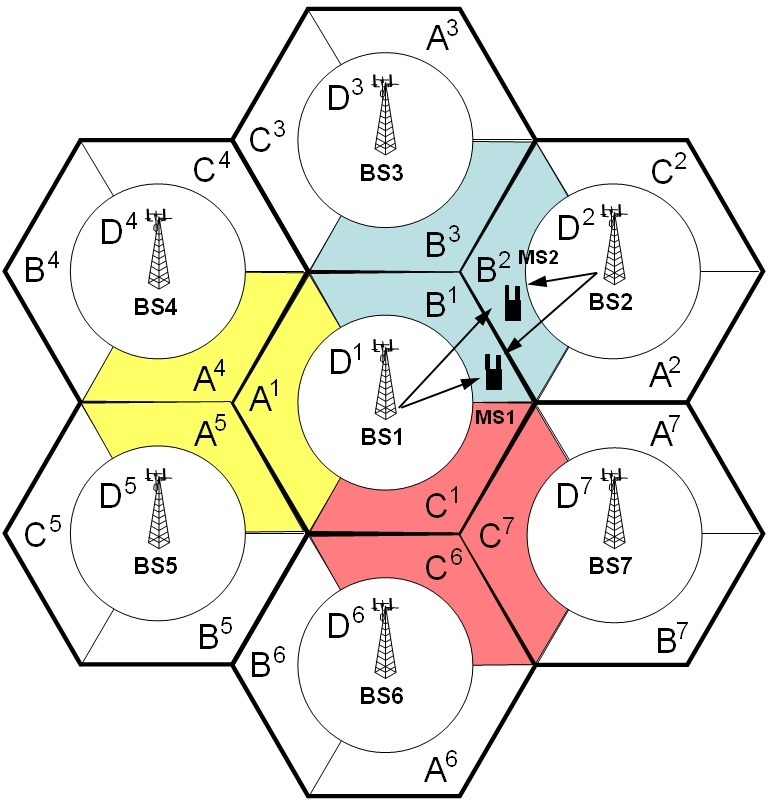
\includegraphics[width=0.48\textwidth]{images/cells_layout.jpg}
    \hfill
    \centering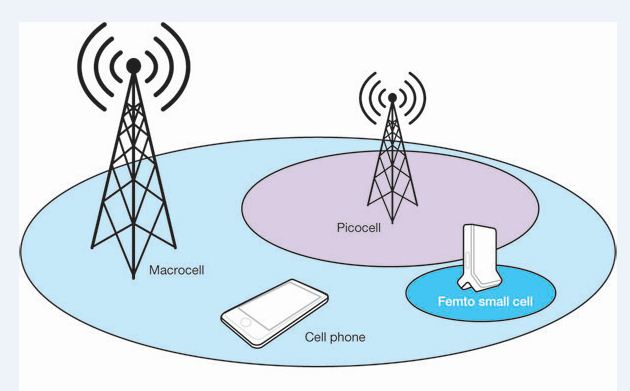
\includegraphics[width=0.48\textwidth]{images/multi_tier.JPG}
  \end{figure}
  \end{center}
\end{frame}

%------------------------------------------------

\begin{frame}
\frametitle{Femtocells}
%\begin{columns}
%\column{0.48\linewidth}
%\column{0.48\linewidth}
\centering
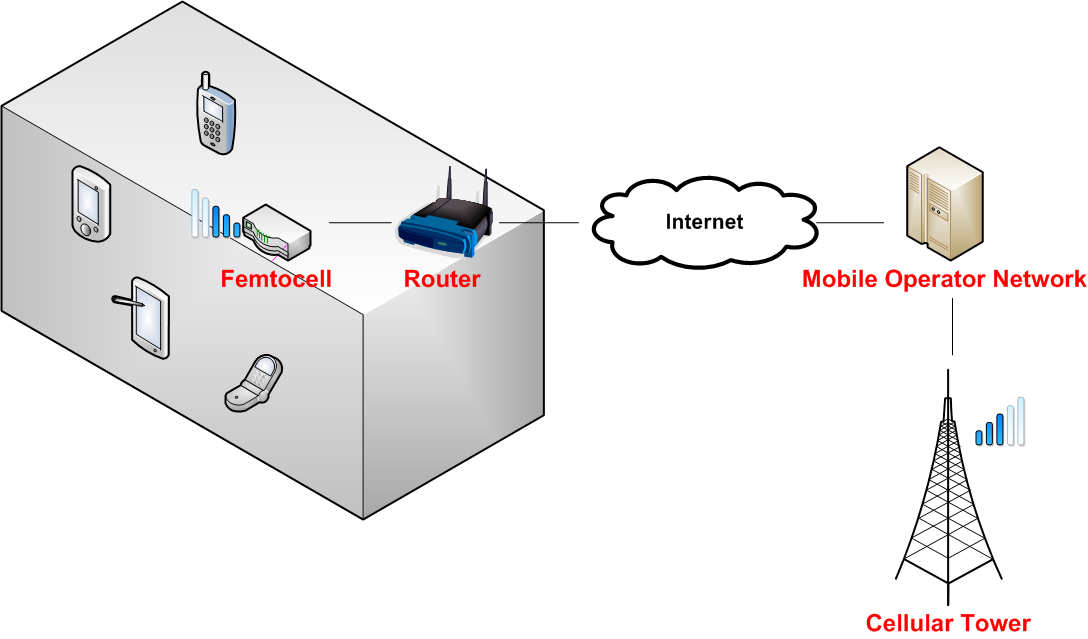
\includegraphics[width=0.8\linewidth]{images/femto.png}
\begin{itemize}
  \item Cheap with small transmission range
  \item Reduce load on Macrocells
  \item Provide service to residential dead zones
\end{itemize}
%\end{columns}
\end{frame}

%------------------------------------------------
\begin{frame}
\frametitle{Interference Problems}

\begin{block}{Inter-cell (Among)}
\begin{itemize}
  \item ICIC (inter-cell interference coordination) is used to resource interference among overlapping edge users
  \item Uses coordination over X2 interface between eNodeB's to enforce scheduling rules
\end{itemize}
\end{block}

\begin{block}{Intra-cell (Within)}
\begin{itemize}
  \item eICIC is still under development and only methods for Pico-cells have been standardized
  \item Femtocell interference is still an area of debate, but will most likely adopt strategies similar to ICIC
  \item Interference among Femtocells is still up for grabs
\end{itemize}
\end{block}

\end{frame}

%------------------------------------------------

\begin{frame}
\frametitle{Current Approaches for Femtocell Interference}
\begin{block}{Split Bands}
\begin{itemize}
  \item Macro users get bands A-C and Femto users get bands D-E
  \item \textbf{Pros}: Simple to implement and no co-channel interference
  \item \textbf{Cos}: Spectrally inefficient
\end{itemize}
\end{block}
%\end{columns}
\begin{block}{Shared Bands}
\begin{itemize}
  \item Both share all bands, Macro transmits deterministic ABS to lower cell edge transmissions
  \item \textbf{Pros}: All users can use all bands
  \item \textbf{Cos}: Co-channel interference, coordination required
\end{itemize}
\end{block}

\end{frame}

%------------------------------------------------
\section{Simulator}
%------------------------------------------------

\begin{frame}
  \frametitle{Overview} % Table of contents slide, comment this block out to remove it
  \tableofcontents % Throughout your presentation, if you choose to use \section{} and \subsection{} commands, these will automatically be printed on this slide as an overview of your presentation
\end{frame}

%------------------------------------------------

\begin{frame}
\frametitle{Goal}
\begin{itemize}
  \item Model interference between Femtocells
  \item Impacts of interference on network
  \item Avoidance with minimal changes to network operation
\end{itemize}
\end{frame}

%------------------------------------------------

\begin{frame}
\frametitle{Scenarios of Interest}
\centering
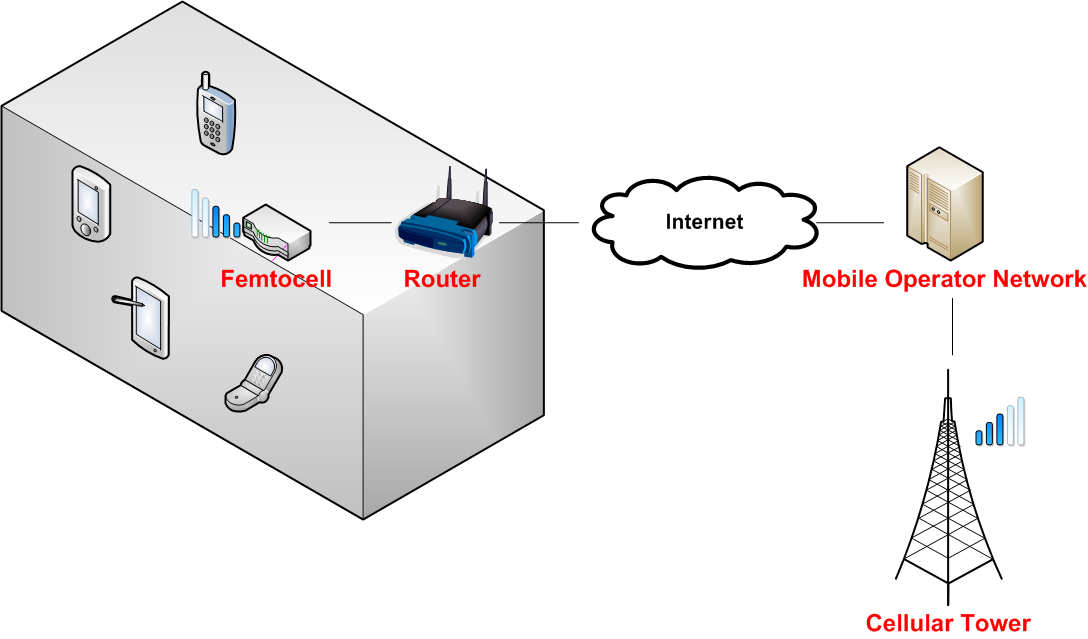
\includegraphics[width=0.8\linewidth]{images/femto.png}
\end{frame}

%------------------------------------------------

\begin{frame}
\frametitle{Working and Tobe Changed}

\begin{block}{Working}
\begin{itemize}
  \item Can simulate N Femtocells with M UE's associate with each cell
  \item Pathloss is based off WINNER Model (Current using indoor only models without walls)
  \item Resource blocks utilization is monitored simulation wide
  \item AP's can have custom positions
  \item Nodes can have customized tasks (aka VOIP, Web, etc...)
  \item Scheduler is Round Robin based (first come first serve)
\end{itemize}
\end{block}

\begin{block}{In progress Work}
  \begin{itemize}
    \item Sensing is non-realistic (Not traditional to LTE)
    \item AP's are assumed synchronized, not realistic
  \end{itemize}
\end{block}

\end{frame}

%------------------------------------------------

\begin{frame}
\frametitle{Modeling Work}
\begin{itemize}
  \item Overall network throughput as nodes increase
  \item Interference characteristics
  \item User statistics
  \item Resource allocation modeling
  \item Smart scheduling
  \item Can sensing be done? Does it provide any advantage?
\end{itemize}
\end{frame}

%------------------------------------------------

\begin{frame}
\frametitle{Scheduler Operation}
\begin{center}
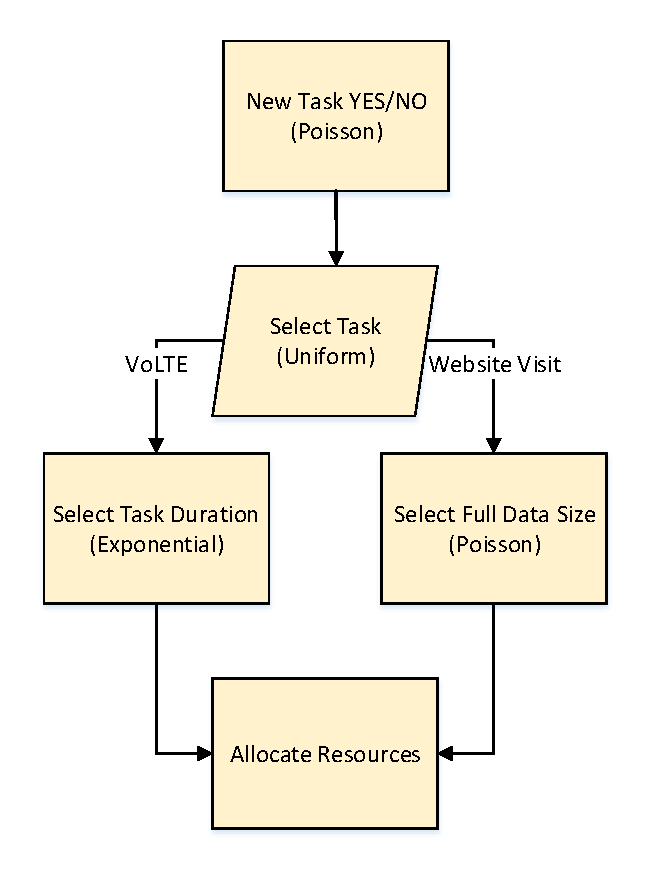
\includegraphics[height=0.65\linewidth]{images/lte_schedular_start.pdf}
\end{center}
\end{frame}

%------------------------------------------------

\begin{frame}
\frametitle{Scheduler Operation}
\begin{center}
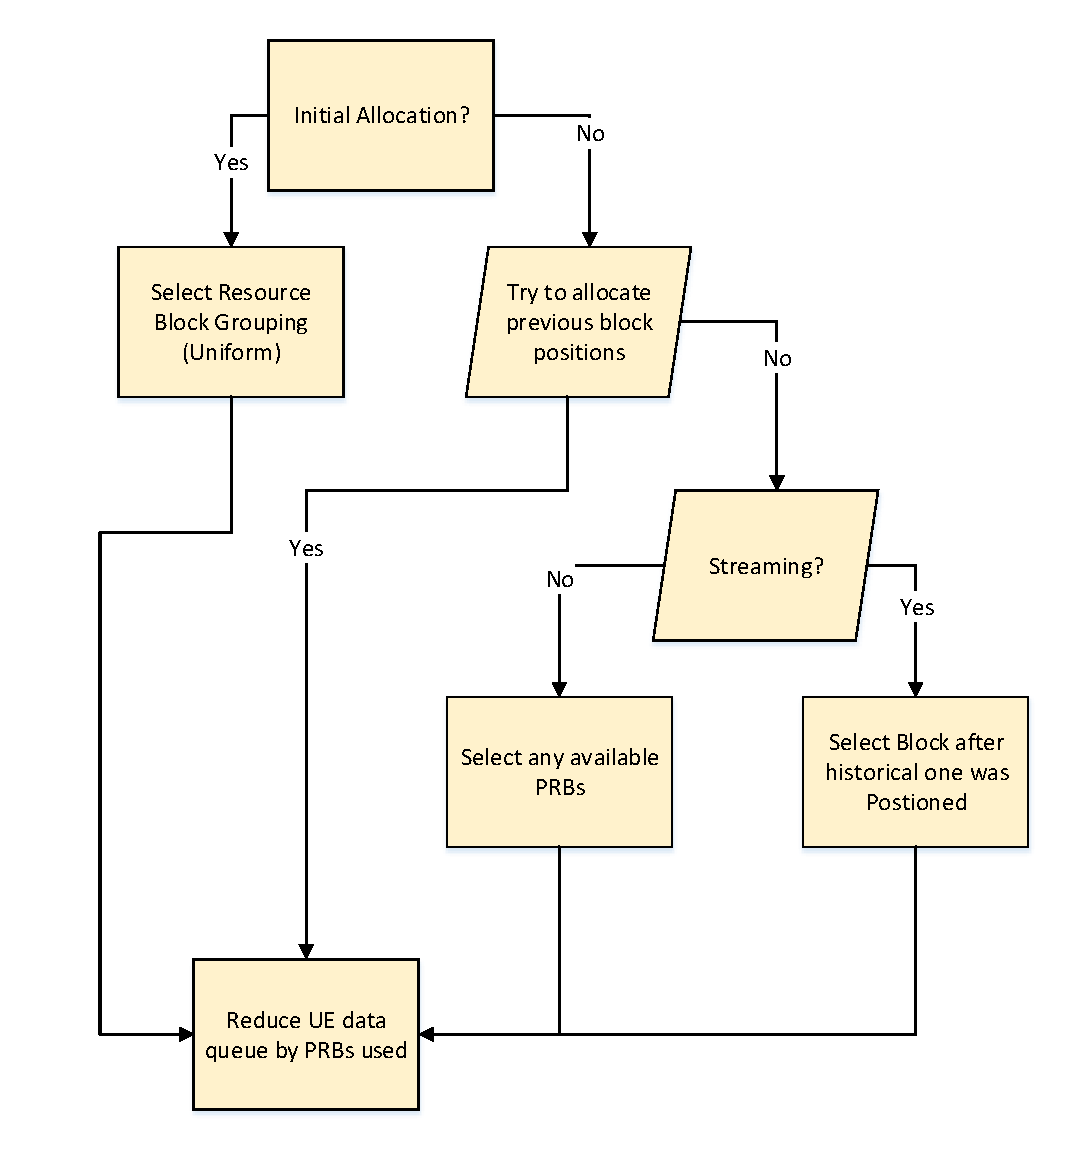
\includegraphics[height=0.65\linewidth]{images/lte_schedular_allocate.pdf}
\end{center}
\end{frame}

%------------------------------------------------

\begin{frame}
\frametitle{Demo}
\Huge{\centerline{Demo}}
\end{frame}

%------------------------------------------------

\begin{frame}
\frametitle{References}
%\footnotesize{
%\begin{thebibliography}{99} % Beamer does not support BibTeX so references must be inserted manually as below
%\bibitem[Smith, 2012]{p1} John Smith (2012)
%\newblock Title of the publication
%\newblock \emph{Journal Name} 12(3), 45 -- 678.
%\end{thebibliography}
%}
\begin{itemize}
%\fontsize{4}{11}\selectfont
\item \url{http://lteuniversity.com/get_trained/expert_opinion1/b/dhar/archive/2010/08/27/one-millisecond-in-the-life-of-an-lte-ue.aspx}
\item \url{http://mwrf.com/site-files/mwrf.com/files/uploads/2012/08/2_1.JPG}
\item \url{http://www.citi.sinica.edu.tw/~rchang/BSC.bmp}
\end{itemize}
\end{frame}

%----------------------------------------------------------------------------------------

\end{document}
